\documentclass{beamer}
\usepackage{tikz}
\usepackage{wasysym}
%:
\title{\\ $ $ \\ $ $ \\ $ $ \\ $ $ \\ Ramsey Theory and Applications to Analysis}
\author{Jake R. Gameroff \\ Honours Research Project \\ June 12, 2024}
\date{}

\begin{document}
{\usebackgroundtemplate{\tikz\node[opacity=0.3, inner sep=0pt] {\includegraphics[width=\paperwidth,height=\paperheight]{/Users/jakeg/Downloads/tree.jpeg}};}
\frame{\titlepage}}

\begin{frame}
\frametitle{Agenda} \textbf{Plan for today:} 
\begin{itemize}
	\item The big picture of Ramsey Theory
	\item Classical examples
		\begin{itemize}
			\item Diagonal Ramsey number + \( R(3)=6 \) 
			\item Van der Waerden numbers
		\end{itemize}
	\item Ramsey's theorem (infinite version)
	\item A \emph{very elegant} application of Ramsey's theorem to analysis
\end{itemize}
\end{frame}

\begin{frame}
\begin{center}
	\Large{\textbf{What is Ramsey Theory?}}
\end{center}
\end{frame}

\begin{frame}
\frametitle{Ramsey Theory: The Big Picture}
{\color{cyan}{\textbf{Ramsey Theory}}} explores the underlying structure emerging in ``large enough" complex systems.\newline

\textbf{Main idea:} In search of a particular kind of structure in a complex system, we ask: \emph{how large must our system be to guarantee the existence of this structure?}
\end{frame}

\begin{frame}
\begin{center}
	\Large{\textbf{Some classical examples}}
\end{center}
\end{frame}

\begin{frame}
\frametitle{Diagonal Ramsey Numbers} The \( k \)'th \textbf{diagonal Ramsey number} \( R(k) \) is the smallest integer \( N \) such that in any colouring of the edges of the complete graph \( K_{N}  \) in either {\color{red}{red}} or {\color{blue}{blue}}, there is always a set of \( k \) vertices joined by all red edges or all blue edges.
\begin{itemize}
	\item \emph{Ramsey's Theorem (finite version):} \( R(k) \) exists for every positive integer \( k \).
	\item \( R(1) = 1 \), \( R(2) = 2 \), \( R(3) = 6 \).
\end{itemize}
\end{frame}

\begin{frame}
    \frametitle{$K_5$ with No Monochrome $K_3$}
    \begin{figure}
        \centering
        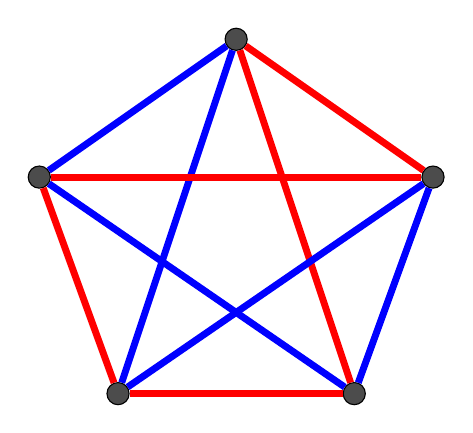
\begin{tikzpicture}[scale=2.5]
            % Define positions of the vertices
          \node[draw, circle, fill=black!70, minimum size=8pt, inner sep=0pt] (v1) at (0, 1) {};
            \node[draw, circle, fill=black!70, minimum size=8pt, inner sep=0pt] (v2) at (-1, 0.3) {};
            \node[draw, circle, fill=black!70, minimum size=8pt, inner sep=0pt] (v3) at (-0.6, -0.8) {};
            \node[draw, circle, fill=black!70, minimum size=8pt, inner sep=0pt] (v4) at (0.6, -0.8) {};
            \node[draw, circle, fill=black!70, minimum size=8pt, inner sep=0pt] (v5) at (1, 0.3) {};


            % draw[line width=2.5pt]edges with specific colors to avoid monochrome K3
            \draw[blue, line width=2.5pt] (v1) -- (v2);
            \draw[blue, line width=2.5pt] (v1) -- (v3);
            \draw[red, line width=2.5pt] (v1) -- (v4);
            \draw[red, line width=2.5pt] (v1) -- (v5);
            \draw[red, line width=2.5pt] (v2) -- (v3);
            \draw[blue, line width=2.5pt] (v2) -- (v4);
            \draw[red, line width=2.5pt] (v2) -- (v5);
            \draw[red, line width=2.5pt] (v3) -- (v4);
            \draw[blue, line width=2.5pt] (v3) -- (v5);
            \draw[blue, line width=2.5pt] (v4) -- (v5);
        \end{tikzpicture}
    \end{figure}
\end{frame}

\begin{frame}
	\frametitle{\( R(3) = 6 \)}
    \begin{figure}
        \centering
        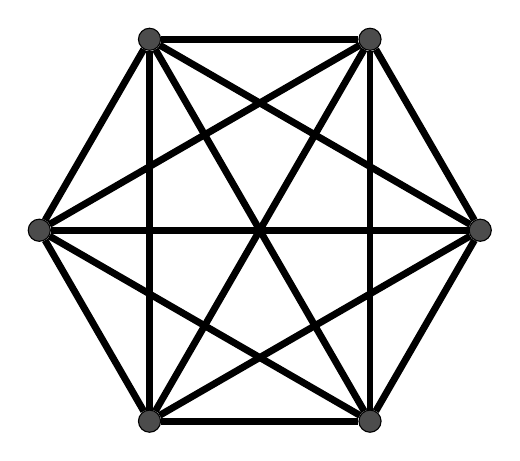
\begin{tikzpicture}[scale=2]
            % Define positions of the vertices in a hexagon
            \foreach \i in {1,...,6} {
                \node[draw, circle, fill=black!70, minimum size=8pt, inner sep=0pt] (v\i) at ({60 * (\i - 1)}:1.4) {};
            }

            \draw[line width=2.5pt](v1) -- (v2);
            \draw[line width=2.5pt](v1) -- (v3);
            \draw[line width=2.5pt](v1) -- (v4);
            \draw[line width=2.5pt](v1) -- (v5);
            \draw[line width=2.5pt](v1) -- (v6);
            \draw[line width=2.5pt](v2) -- (v3);
            \draw[line width=2.5pt](v2) -- (v4);
            \draw[line width=2.5pt](v2) -- (v5);
            \draw[line width=2.5pt](v2) -- (v6);
            \draw[line width=2.5pt](v3) -- (v4);
            \draw[line width=2.5pt](v3) -- (v5);
            \draw[line width=2.5pt](v3) -- (v6);
            \draw[line width=2.5pt](v4) -- (v5);
            \draw[line width=2.5pt](v4) -- (v6);
            \draw[line width=2.5pt](v5) -- (v6);
        \end{tikzpicture}
    \end{figure}
\end{frame}

\begin{frame}
	\frametitle{\( R(3) = 6 \)}
    \begin{figure}
        \centering
        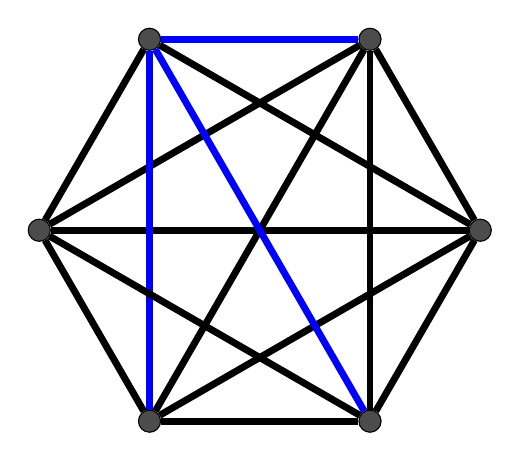
\begin{tikzpicture}[scale=2]
            % Define positions of the vertices in a hexagon
            \foreach \i in {1,...,6} {
                \node[draw, circle, fill=black!70, minimum size=8pt, inner sep=0pt] (v\i) at ({60 * (\i - 1)}:1.4) {};
            }

            % draw[line width=2.5pt]edges with specific colors to avoid monochrome K3
            \draw[line width=2.5pt](v1) -- (v2);
            \draw[line width=2.5pt](v1) -- (v3);
            \draw[line width=2.5pt](v1) -- (v4);
            \draw[line width=2.5pt](v1) -- (v5);
            \draw[line width=2.5pt](v1) -- (v6);
	    \draw[blue, line width=2.5pt](v2) -- (v3);
            \draw[line width=2.5pt](v2) -- (v4);
            \draw[line width=2.5pt](v2) -- (v5);
            \draw[line width=2.5pt](v2) -- (v6);
            \draw[line width=2.5pt](v3) -- (v4);
	    \draw[blue, line width=2.5pt] (v3) -- (v5);
	    \draw[blue, line width=2.5pt] (v3) -- (v6);
            \draw[line width=2.5pt](v4) -- (v5);
            \draw[line width=2.5pt](v4) -- (v6);
            \draw[line width=2.5pt](v5) -- (v6);
        \end{tikzpicture}
    \end{figure}
\end{frame}

\begin{frame}
	\frametitle{\( R(3) = 6 \)}
    \begin{figure}
        \centering
        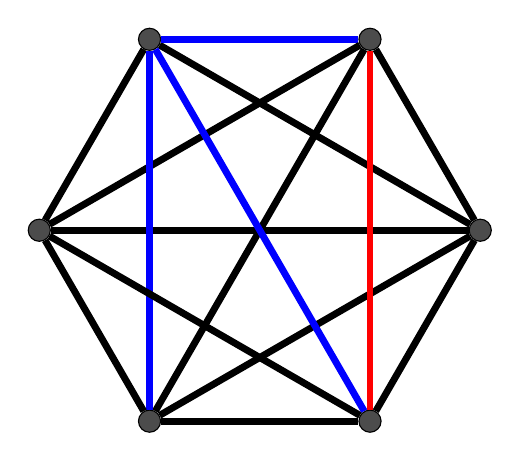
\begin{tikzpicture}[scale=2]
            % Define positions of the vertices in a hexagon
            \foreach \i in {1,...,6} {
                \node[draw, circle, fill=black!70, minimum size=8pt, inner sep=0pt] (v\i) at ({60 * (\i - 1)}:1.4) {};
            }

            % draw[line width=2.5pt]edges with specific colors to avoid monochrome K3
            \draw[line width=2.5pt](v1) -- (v2);
            \draw[line width=2.5pt](v1) -- (v3);
            \draw[line width=2.5pt](v1) -- (v4);
            \draw[line width=2.5pt](v1) -- (v5);
            \draw[line width=2.5pt](v1) -- (v6);
	    \draw[blue, line width=2.5pt](v2) -- (v3);
            \draw[line width=2.5pt](v2) -- (v4);
            \draw[line width=2.5pt](v2) -- (v5);
            \draw[red, line width=2.5pt](v2) -- (v6);
            \draw[line width=2.5pt](v3) -- (v4);
	    \draw[blue, line width=2.5pt] (v3) -- (v5);
	    \draw[blue, line width=2.5pt] (v3) -- (v6);
            \draw[line width=2.5pt](v4) -- (v5);
            \draw[line width=2.5pt](v4) -- (v6);
            \draw[line width=2.5pt](v5) -- (v6);
        \end{tikzpicture}
    \end{figure}
\end{frame}
\begin{frame}
	\frametitle{\( R(3) = 6 \)}
    \begin{figure}
        \centering
        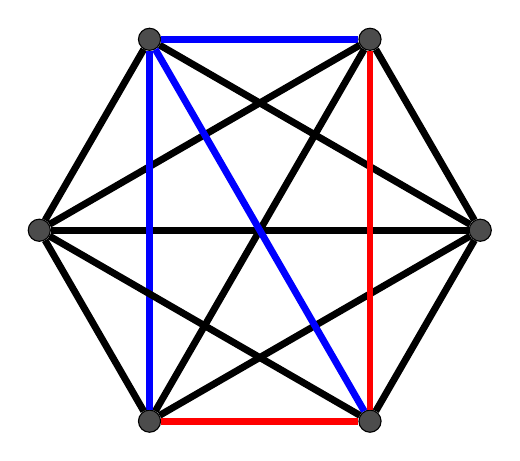
\begin{tikzpicture}[scale=2]
            % Define positions of the vertices in a hexagon
            \foreach \i in {1,...,6} {
                \node[draw, circle, fill=black!70, minimum size=8pt, inner sep=0pt] (v\i) at ({60 * (\i - 1)}:1.4) {};
            }

            % draw[line width=2.5pt]edges with specific colors to avoid monochrome K3
            \draw[line width=2.5pt](v1) -- (v2);
            \draw[line width=2.5pt](v1) -- (v3);
            \draw[line width=2.5pt](v1) -- (v4);
            \draw[line width=2.5pt](v1) -- (v5);
            \draw[line width=2.5pt](v1) -- (v6);
	    \draw[blue, line width=2.5pt](v2) -- (v3);
            \draw[line width=2.5pt](v2) -- (v4);
            \draw[line width=2.5pt](v2) -- (v5);
            \draw[red, line width=2.5pt](v2) -- (v6);
            \draw[line width=2.5pt](v3) -- (v4);
	    \draw[blue, line width=2.5pt] (v3) -- (v5);
	    \draw[blue, line width=2.5pt] (v3) -- (v6);
            \draw[line width=2.5pt](v4) -- (v5);
            \draw[line width=2.5pt](v4) -- (v6);
            \draw[red, line width=2.5pt](v5) -- (v6);
        \end{tikzpicture}
    \end{figure}
\end{frame}

\begin{frame}
	\frametitle{\( R(3) = 6 \)}
    \begin{figure}
        \centering
        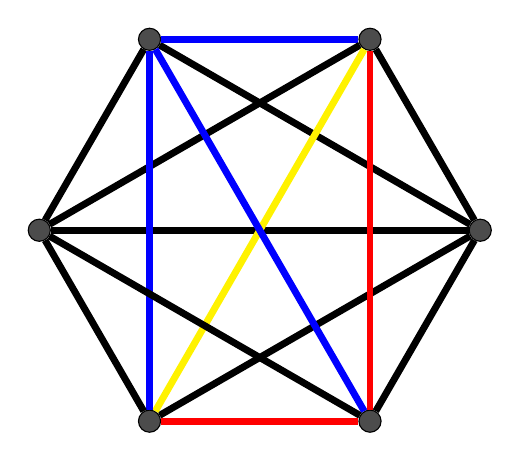
\begin{tikzpicture}[scale=2]
            % Define positions of the vertices in a hexagon
            \foreach \i in {1,...,6} {
                \node[draw, circle, fill=black!70, minimum size=8pt, inner sep=0pt] (v\i) at ({60 * (\i - 1)}:1.4) {};
            }

            % draw[line width=2.5pt]edges with specific colors to avoid monochrome K3
            \draw[line width=2.5pt](v1) -- (v2);
            \draw[line width=2.5pt](v1) -- (v3);
            \draw[line width=2.5pt](v1) -- (v4);
            \draw[line width=2.5pt](v1) -- (v5);
            \draw[line width=2.5pt](v1) -- (v6);
	    \draw[blue, line width=2.5pt](v2) -- (v3);
            \draw[line width=2.5pt](v2) -- (v4);
            \draw[yellow, line width=2.5pt](v2) -- (v5);
            \draw[red, line width=2.5pt](v2) -- (v6);
            \draw[line width=2.5pt](v3) -- (v4);
	    \draw[blue, line width=2.5pt] (v3) -- (v5);
	    \draw[blue, line width=2.5pt] (v3) -- (v6);
            \draw[line width=2.5pt](v4) -- (v5);
            \draw[line width=2.5pt](v4) -- (v6);
            \draw[red, line width=2.5pt](v5) -- (v6);
        \end{tikzpicture}
    \end{figure}
\end{frame}

\begin{frame}
	\frametitle{Van der Waerden Numbers} For \( r, k \in \mathbb{N} \), the \textbf{Van der Waerden number} \( W(k,r) \) is the smallest integer \( N \) such that in any coloring of \( [n] \) in \( k \) colors there is a set of \( r \) monochromatic integers in arithmetic progression.
\begin{itemize}
	\item \emph{Van der Waerden's Theorem:} \( W(k,r) \) exists for all positive integers \( r,k\).
	\item Positive integers \( a_1, a_2, \hdots , a_{r}  \) are in \textbf{arithmetic progression} if there is an integer \( d \geq 0 \) such that the difference of consecutive terms is \( d \); that is, for \( 1 \leq k \leq n - 1 \), \[ a_{k+1} - a_{k} = d. \]
\end{itemize}
\end{frame}

\begin{frame}
\begin{center}
	\Large{\textbf{Ramsey's Theorem (infinite version)}}
\end{center}
\end{frame}

\begin{frame}
\frametitle{Notation} \textbf{We fix some notation:} For a set \( X \), let \( [X]^{2} \) denote the family of all two element subsets of \( X \), i.e. the \emph{edges} between points in \( X \).
\end{frame}

\begin{frame}
	\frametitle{Ramsey's Theorem (infinite version)} In every coloring of \( [\mathbb{N}]^{2}  \) in either {\color{red}{red}} or {\color{blue}{blue}} there is an infinite subset \( A \) of \( \mathbb{N} \) such that all edges in \( [A]^{2}  \) are the same color.
\end{frame}

\begin{frame}
	\frametitle{Proof of Ramsey's Theorem (infinite version)} \textbf{Statement:} In every red-blue coloring of \( [\mathbb{N}]^{2}  \) there is an infinite subset \( A \) of \( \mathbb{N} \) such that all edges in \( [A]^{2}  \) are the same color. \newline
\begin{proof}
Set \( A_0 = \mathbb{N}  \), fix \( x_0 \in A_0 \). By Pigeonhole, \( \exists c_0 \in \{ {\color{red}{\mbox{red}}}, {\color{blue}{\mbox{blue}}} \}  \) with \( A_1 = \{ x \in A_0 : \{ x_0, x \} \mbox{ has color \( c_0 \)} \}  \) infinite. Fix \( x_1 \in A_1 \) and apply the same argument: \( \exists c_1 \in \{ {\color{red}{\mbox{red}}}, {\color{blue}{\mbox{blue}}} \}  \) so that the set \( A_2 = \{ x \in A_1 : \{ x_1, x \} \mbox{ has color \( c_1 \)} \}  \) is infinite. Continue to obtain the following for every \( k \in \mathbb{N} \):
\begin{enumerate}
	\item \( x_{k} \in A_{k}  \),
	\item \( A_{k+1} \subseteq A_{k}  \),
	\item \( \forall x \in A_{k+1} : \{ x_{k} , x \}  \) has color \( c_{k}  \).
\end{enumerate}
Let \( c \in  \{ {\color{red}{\mbox{red}}}, {\color{blue}{\mbox{blue}}} \}  \) be such that \( c = c_{k}  \) for infinitely many \( k \). Then \( A = \{ x_{k} : c_{k} = c \}  \) edges only with color \( c \).
\end{proof}
\end{frame}

\begin{frame}
    \begin{figure}
        \centering
        \begin{minipage}{0.48\textwidth}
            \centering
            \includegraphics[width=\textwidth]{/Users/jakeg/Desktop/RamseyTalk/Presentation/images/1.png}
        \end{minipage}
        \hfill
        \begin{minipage}{0.48\textwidth}
            \centering
            \includegraphics[width=\textwidth]{/Users/jakeg/Desktop/RamseyTalk/Presentation/images/2.png}
        \end{minipage}
    \end{figure}
\end{frame}




\begin{frame}
\frametitle{A Lemma} We need the following lemma: \\

\textbf{Lemma.} \emph{Every sequence \( (x_{n}) \) in \( \mathbb{R} \) has a monotone subsequence.}
\begin{proof}
	Given natural numbers \( n , m  \) with \( n < m \), color the edge \( e = \{n , m \}  \) {\color{red}{red}} if \( x_{n} \leq x_{m}  \) and color \( e \) {\color{blue}{blue}} otherwise.
	\begin{itemize}
		\item From Ramsey's Theorem, there is an infinite subset \( A \subseteq \mathbb{N}  \) such that \( [A]^{2}  \) is either red or blue. Write \( A = (n_{k} )_{k \in \mathbb{N} }  \) so that \( n_k \leq n_{k+1} \) for each \( k \in \mathbb{N}  \).
		\item Then the subsequence \( (x_{n_{k} })_{k \in \mathbb{N}}  \) is monotone: it is non-decreasing if \( [A]^{2}  \) is red and it is non-increasing if \( [A]^{2}  \) is blue.

		
	\end{itemize}
\end{proof}
\end{frame}

\begin{frame}
	\frametitle{Proving The Bolzano-Weierstrass Theorem} \textbf{Theorem} (Bolzano-Weierstrass)\textbf{.} \emph{Every bounded sequence \( (x_{n}) \) of real numbers has a convergent subsequence.}
\begin{proof}
From the lemma, \( (x_{n}) \) has a monotone subsequence which is bounded as \( (x_{n}) \) is. Since bounded monotone sequences converge, this subsequence is convergent.
\end{proof}
\end{frame}

\begin{frame}
	\frametitle{Acknowledgements}

\begin{itemize}
	\item I would like to give my most sincere thanks Professor Jakobson for his kindness in helping me prepare this presentation. 
	\item I also dearly thank Professor Anush Tserunyan for teaching me about this clever combinatorial proof of the BW theorem. I learnt this during my first semester in one of her Math 254 lectures, and it has stuck with me ever since.
\end{itemize}

\end{frame}

\begin{frame}
	\begin{center}
		{\Large \color{cyan}{\textbf{Thank you all for listening to my talk!}}} \newline \newline
		\large Any and all questions are appreciated. $\smiley$
	\end{center}
\end{frame}

\end{document}


%\textbf{Reminder:} \( x_{n-1}  \) has infinitely-many edges with color \( c_{n-1}  \) and \[ A_{n} = \{ x \in A_{n - 1} : x_{n-1} < x \mbox{ and } \{ x_{n-1} , x \} \mbox{ has color } c_{n-1}  \}  \]
